\documentclass{article}
\usepackage{amsmath, amssymb, amsthm, graphicx}

\title{Chapter 2 Section 1}
\author{Andrew Taylor}
\date{March 26 2022}
\newtheorem{theorem}{Theorem}
\newtheorem{problem}{Problem}
\newtheorem*{solution}{Solution}

\begin{document}
\maketitle

\begin{problem}
Imagine yourself cruising in the Mediterranean as a crew member on a French coast goard boat, looking for evildoers. Periodically, your boat radios its position to headquarters in Marseille. You expect that communications will be intercepted. So, before you broadcast anything, you have to transform the actual position of the boat,

\begin{align*}
\begin{bmatrix}
x1 \\ x2
\end{bmatrix}
\end{align*}

($x_{1}$ for Eastern longitude, $x_{2}$ for Northern latitude), into an encoded position

\begin{align*}
\begin{bmatrix}
y_{1} \\ y_{2}
\end{bmatrix}
\end{align*}

You use the following code:

\begin{align*}
y_{1} &= x_{1} + 3x_{2} \\
y_{2} &= 2x_{2} + 5x_{2}
\end{align*}

For example, when the actual position of your boat is $5^\circ E$, $42^\circ N$, or

\begin{align*}
\vec{x} = \begin{bmatrix} x_{1} \\ x_{2} \end{bmatrix} = \begin{bmatrix} 5 \\ 42 \end{bmatrix}
\end{align*}

your encoded position will be 

\begin{align*}
\vec{y} 
&= \begin{bmatrix} y_{1} \\ y_{2} \end{bmatrix} \\
&= \begin{bmatrix} 
x_{1} + 3x_{2} \\ 
2x_{1} + 5x_{2} 
\end{bmatrix} \\
&= \begin{bmatrix}
5 + 3 * 42 \\ 2 * 5 + 5 * 42
\end{bmatrix} \\
&= \begin{bmatrix} 
131 \\ 220
\end{bmatrix}
\end{align*}

The coding transformation can be represented as

\begin{align*}
\vec{y} 
&= \begin{bmatrix} y_{1} \\ y_{2} \end{bmatrix} \\
&= \begin{bmatrix} 1 & 3 \\ 2 & 5  \end{bmatrix} \\
&= \begin{bmatrix} x_{1} \\ x_{2} \end{bmatrix}
\end{align*}

Figure 1

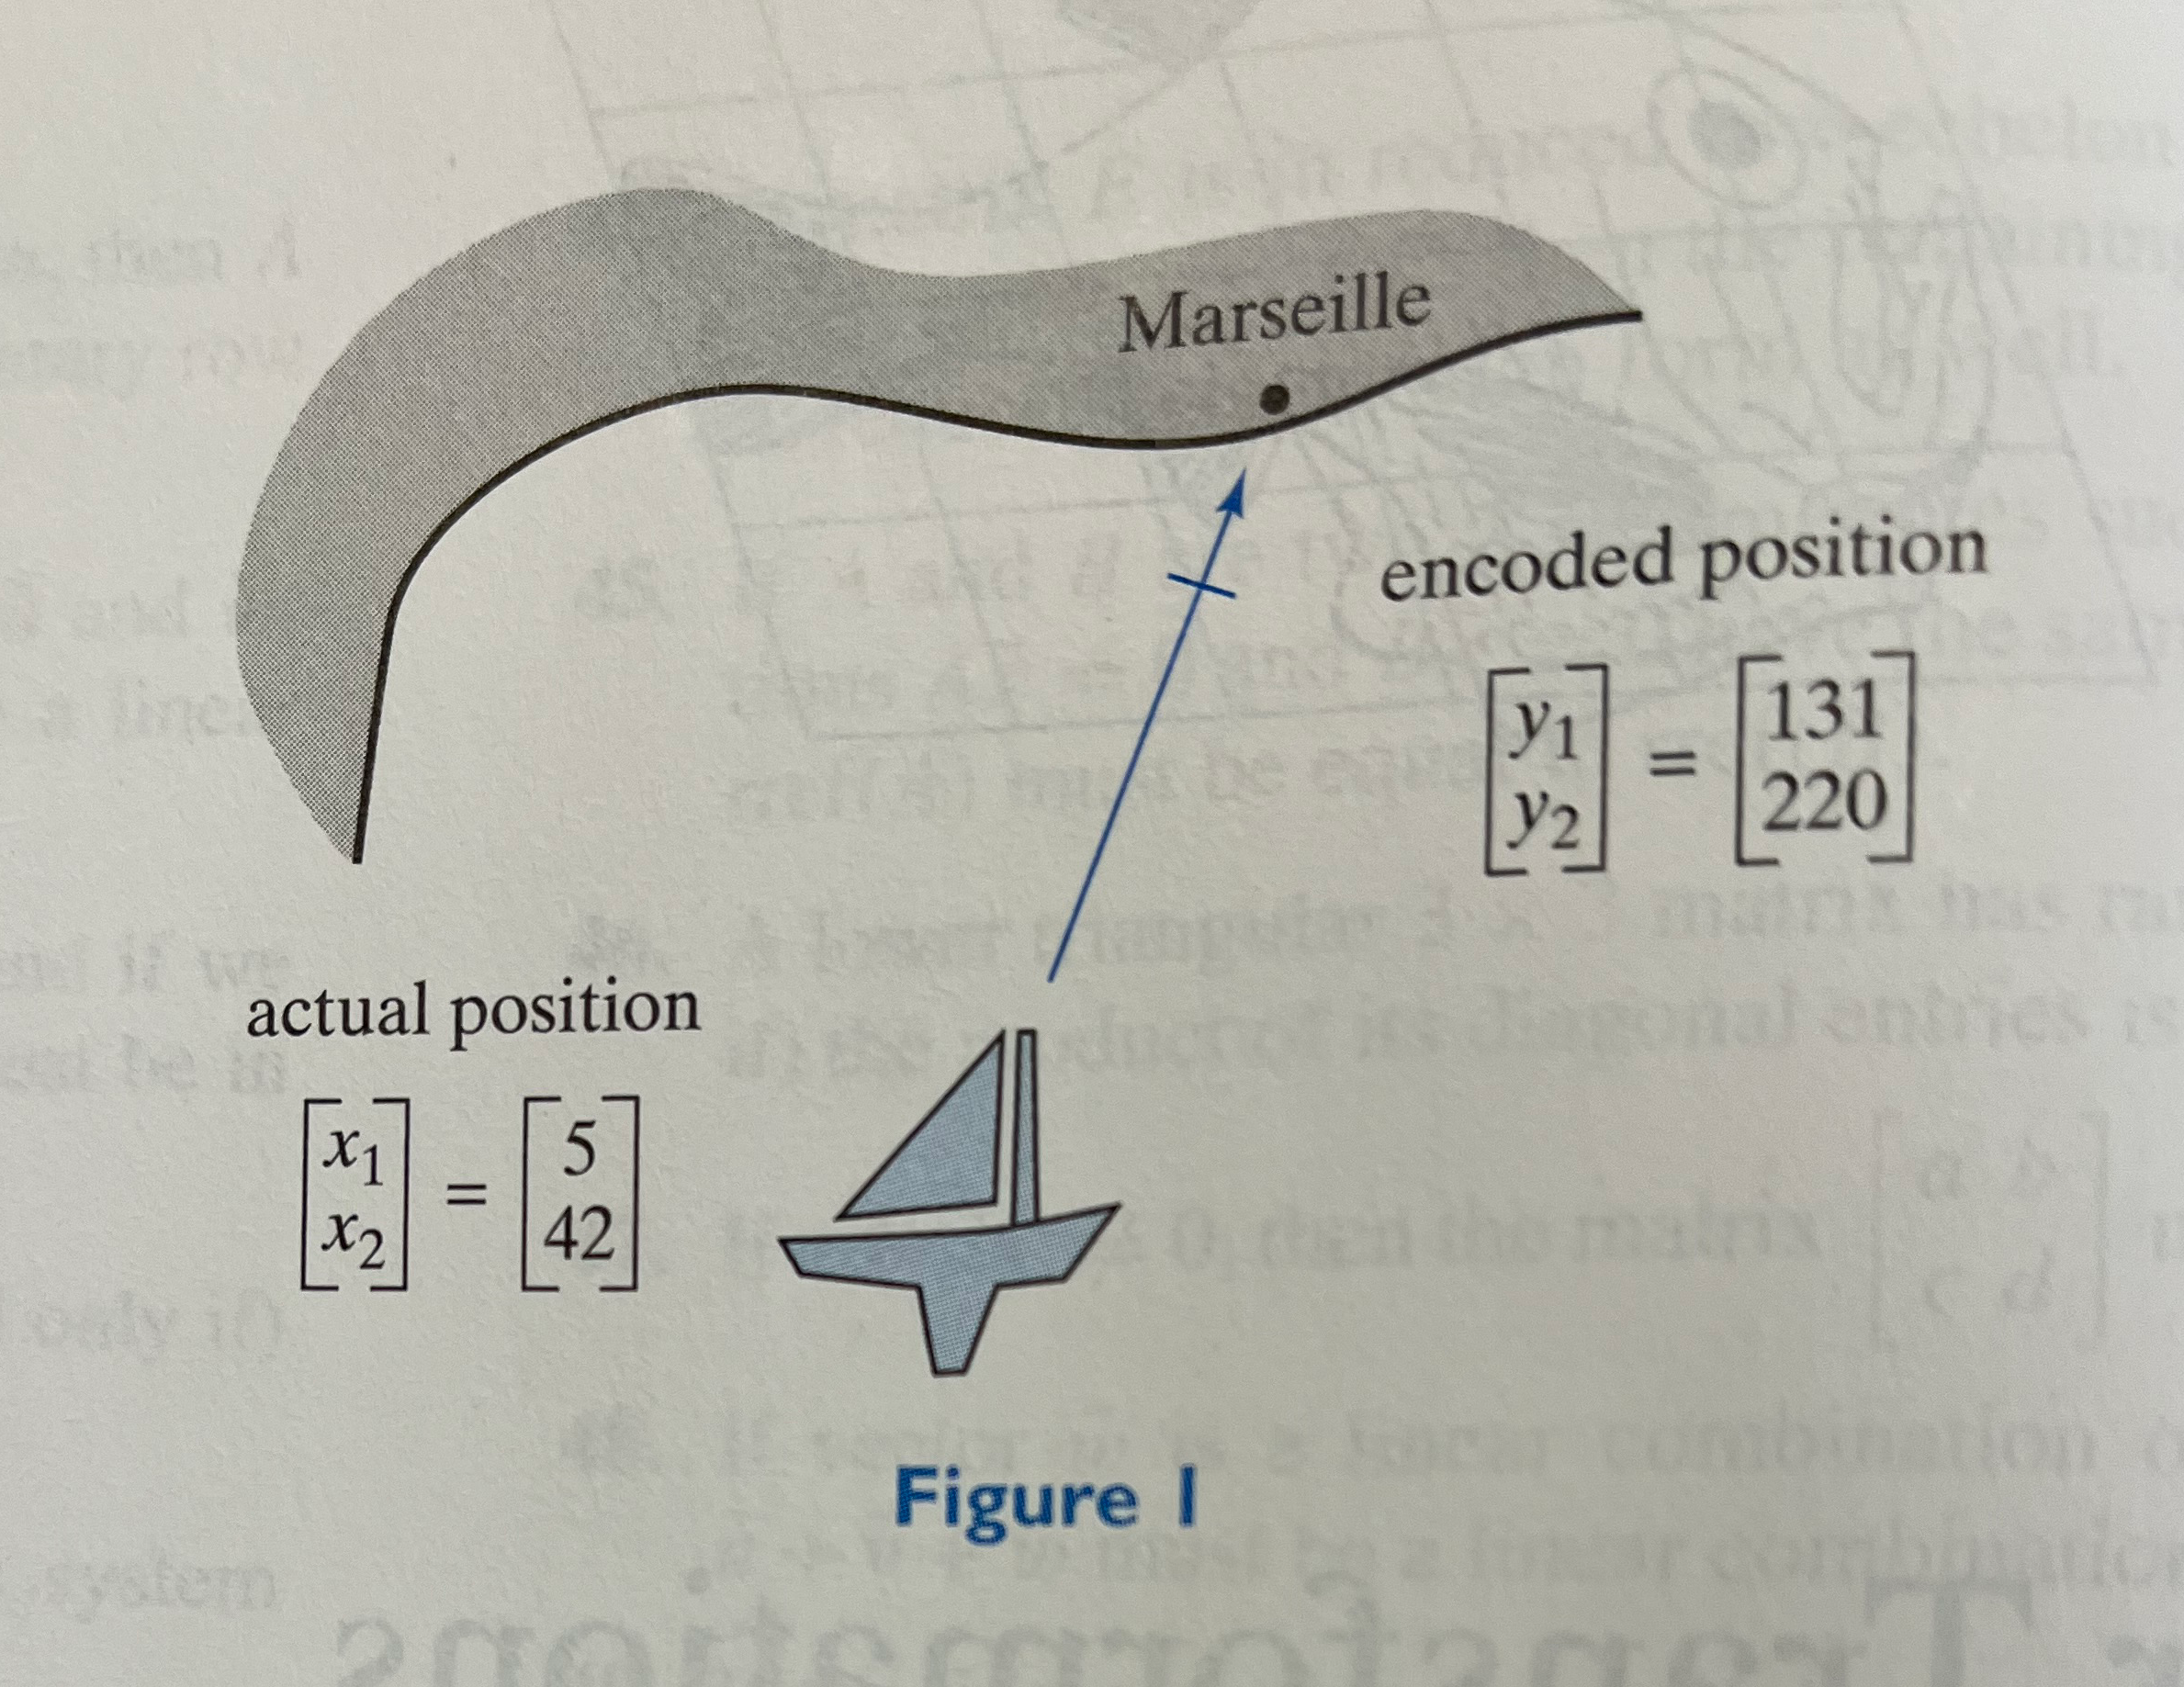
\includegraphics[scale=0.1]{ch2sec1fig1} 


As the ship reaches a new position, the sailor on duty at headquarters in Marseille receives the encoded message

\begin{align*}
\vec{b} = \begin{bmatrix} 133 \\ 223 \end{bmatrix} 
\end{align*}

He must determine the actual position of the boat. He will have to solve the linear system

\begin{align*}
A\vec{x} = \vec{b}
\end{align*}

or, more explicitly,

\begin{align*}
\begin{vmatrix}
x_{1} + 3x_{2} = 133 \\
2x_{1} + 5x_{2} = 223
\end{vmatrix}
\end{align*}

Here is his solution. Is it correct?

\begin{align*}
\vec{x} = \begin{bmatrix} x_{1} \\ x_{2} \end{bmatrix} = \begin{bmatrix} 4 \\ 43 \end{bmatrix}
\end{align*}

\end{problem}

\begin{solution}

We can use elementary row operations to solve the system. Remember, the elementary row operations are subtracting a multiple of a row, dividing a row by a scalar, and swapping rows.

\begin{align*}
& \begin{bmatrix}
1 & 3 & 133 \\
2 & 5 & 223
\end{bmatrix} \\
&\begin{bmatrix}
1 & 3 & 133 \\
0 & -1 & -43
\end{bmatrix} \\
& \begin{bmatrix}
1 & 3 & 133 \\
0 & 1 & 43
\end{bmatrix} \\
& \begin{bmatrix}
1 & 0 & 4 \\
0 & 1 & 43
\end{bmatrix}
\end{align*}

Thus his solution is correct. The solution is 

\begin{align*}
\vec{x} = \begin{bmatrix} x_{1} \\ x_{2} \end{bmatrix} = \begin{bmatrix} 4 \\ 43 \end{bmatrix}
\end{align*}

What we really did is we applied the linear transformation (the code we were given) to the encoded message, to get the actual coordinates.

\end{solution}

Consider the transformations from $\mathbb{R}^3$ to $\mathbb{R}^3$. Which of these transformations are linear?

\begin{problem}

\begin{align*}
y_{1} &= 2x_{2} \\
y_{2} &= x_{2} + 2 \\
y_{3} &= 2x_{2}
\end{align*}

\end{problem}

\begin{solution}
Let $T$ be the linear transformation, and let $\vec{v}$ and $\vec{w}$ be vectors in $\mathbb{R}^3$.

\begin{align*}
& T(\vec{v} + \vec{w}) \\
&= T((v_{1}, v_{2}, v_{3}) + (w_{1}, w_{2}, w_{3})) \\
&= T((v_{1} + w_{1}, v_{2} + w_{2}, v_{3} + w_{3})) \\
&= (2(v_{2} + w_{2}), v_{2} + w_{2} + 2, 2(v_{2} + w_{2}))
\end{align*}

\begin{align*}
& T(\vec{v}) + T(\vec{w}) \\
&= T((v_{1}, v_{2}, v_{3})) + T((w_{1}, w_{2}, w_{3})) \\
&= (2(v_{2}), v_{2} + 2, 2(v_{2})) + (2(w_{2}), w_{2} + 2, 2(w_{2})) \\
&= (2(v_{2} + w_{2}), v_{2} + w_{2} + 2, 2(v_{2} + w_{2}))
\end{align*}

Thus 

\begin{align*}
T(\vec{v} + \vec{w}) = T(\vec{v}) + T(\vec{w})
\end{align*}

Let $k$ be a scalar in $\mathbb{R}$.

\begin{align*}
& T(k\vec{v}) \\
&= T((kv_{1}, kv_{2}, kv_{3})) \\
&= (2kv_{2}, kv_{2} + 2, 2kv_{2}) 
\end{align*}

\begin{align*}
& kT(\vec{v}) \\
&= kT((v_{1}, v_{2}, v_{3})) \\
&= k(2v_{2}, v_{2} + 2, 2v_{2}) \\
&= (2kv_{2}, kv_{2} + 2, 2kv_{2}) 
\end{align*}

Thus 

\begin{align*}
T(k\vec{v}) = kT(\vec{v})
\end{align*}

T satisfies the two properties of a linear transformation, so T is a linear transformation.

\end{solution}

\begin{problem}

\begin{align*}
y_{1} &= 2x_{2} \\
y_{2} &= 3x_{3}  \\
y_{3} &= x_{1}
\end{align*}

\end{problem}

\begin{solution}
Let T be the linear transformation, $\vec{v}$ and $\vec{w}$ be vectors in $\mathbb{R}^{3}$.

\begin{align*}
& T(\vec{v} + \vec{w}) \\ 
&= T((v_{1}, v_{2}, v_{3}) + (w_{1}, w_{2}, w_{3})) \\
&= T((v_{1} + w_{1}, v_{2} + w_{2}, v_{3} + w_{3})) \\
&= (2(v_{2} + w_{2}), 3(v_{3} + w_{3}), v_{1} + w_{1})
\end{align*}

\begin{align*}
& T(\vec{v}) + T(\vec{w}) \\
&= (2v_{2}, 3v_{3}, v_{1}) + (2w_{2}, 3w_{3}, w_{1}) \\
&= (2(v_{2} + w_{2}), 3(v_{3} + w_{3}), v_{1} + w_{1})
\end{align*}

Thus

\begin{align*}
T(\vec{v}) + T(\vec{w}) = T(\vec{v} + \vec{w})
\end{align*}

Let $k$ be a scalar in the reals.

\begin{align*}
& T(k\vec{v}) \\
&= T((kv_{1}, kv_{2}, kv_{3}) \\
&= (2kv_{2}, 3kv_{3}, kv_{1}) 
\end{align*}

\begin{align*}
& kT(\vec{v}) \\
&= k(2v_{2}, 3v_{3}, v_{1}) \\
&= (2kv_{2}, 3kv_{3}, kv_{1})
\end{align*}

Thus 

\begin{align*}
T(k\vec{v}) = kT(\vec{v})
\end{align*}

Therefore T is a linear transformation, because it satisfies both requirements of a linear transformation.

\end{solution}

\begin{problem}

\begin{align*}
y_{1} &= x_{2} - x_{3} \\
y_{2} &= x_{1} x_{3}  \\
y_{3} &= x_{1} - x_{2}
\end{align*}

\end{problem}

\begin{solution}
Let T be the linear transformation and let $\vec{v}$ and $\vec{w}$ be vectors in $\mathbb{R}^3$.

\begin{align*}
& T(\vec{v} + \vec{w}) \\
&= T((v_{1}, v_{2}, v_{3}) + (w_{1}, w_{2}, w_{3})) \\ 
&= T((v_{1} + w_{1}, v_{2} + w_{2}, v_{3} + w_{3})) \\
&= (v_{2} + w_{2} - v_{3} - w_{3}, (v_{1} + w_{1}) * (v_{3} + w_{3}), v_{1} + w_{1} - v_{2} - w_{2}) 
\end{align*}

\begin{align*}
& T(\vec{v}) + T(\vec{w}) \\
&= (v_{2} - v_{3}, v_{1} * v_{3}, v_{1} - v_{2}) + (w_{2} - w_{3}, w_{1} * w_{3}, w_{1} - w_{2}) \\
&= (v_{2} - v_{3} + w_{2} - w_{3}, v_{1} * v_{3} + w_{1} * w_{3}, v_{1} - v_{2} + w_{1} - w_{2}) 
\end{align*}

The two vectors are not equal, therefore T is not a linear transformation. In other words,

\begin{align*}
T(\vec{v}) + T(\vec{w}) \neq T(\vec{v} + \vec{w})
\end{align*}

so T is not a linear transformation.
\end{solution}

\begin{problem}

Find the matrix of the linear transformation

\begin{align*}
y_{1} &= 9x_{1} + 3x_{2} - 3x_{3} \\
y_{2} &= 2x_{1} - 9x_{2} + x_{3} \\
y_{3} &= 4x_{1} - 9x_{2} - 2x_{3} \\ 
y_{4} &= 5x_{1} + x_{2} + 5x_{3}
\end{align*}

\end{problem}

\begin{solution}

\begin{align*}
\vec{y} &= A \vec{x} \\
&= \begin{pmatrix}
9 & 3 & -3 \\
2 & -9 & 1 \\
4 & -9 & -2 \\
5 & 1 & 5 
\end{pmatrix}
\vec{x} \\
&= \begin{pmatrix}
9 & 3 & -3 \\
2 & -9 & 1 \\
4 & -9 & -2 \\
5 & 1 & 5 
\end{pmatrix}
\begin{pmatrix}
x_{1} \\ x_{2} \\ x_{3}
\end{pmatrix}
\end{align*}

We see that the matrix has four rows and three columns, transforming a three-dimensional vector into a four-dimensional vector.

\end{solution}

\begin{problem}
Consider the linear transformation T from $\mathbb{R}^3$ to $\mathbb{R}^2$ with 

\begin{align*}
T \begin{bmatrix} 1 \\ 0 \\ 0 \end{bmatrix} &= \begin{bmatrix} 7 \\ 1 \end{bmatrix}, \\
T \begin{bmatrix} 0 \\ 1 \\ 0 \end{bmatrix} &= \begin{bmatrix} 6 \\ 9 \end{bmatrix}, \\
T \begin{bmatrix} 0 \\ 0 \\ 1 \end{bmatrix} &= \begin{bmatrix} -13 \\ 17 \end{bmatrix}
\end{align*}

Find the matrix A of T.
\end{problem}

\begin{solution}
We can write the equation

\begin{align*}
\begin{pmatrix}
7 \\ 1
\end{pmatrix}
&= A \begin{pmatrix} 1 \\ 0 \\ 0 \end{pmatrix} \\
\begin{pmatrix}
7 \\ 1
\end{pmatrix}
&= 
\begin{pmatrix} 
c_{1} & c_{2} & c_{3} \\
d_{1} & d_{2} & d_{3}
\end{pmatrix}
\begin{pmatrix} 1 \\ 0 \\ 0 \end{pmatrix}
\end{align*}

So $c_{1} = 7$ and $d_{1} = 1$

\begin{align*}
\begin{pmatrix}
6 \\ 9
\end{pmatrix}
&= A \begin{pmatrix} 0 \\ 1 \\ 0 \end{pmatrix} \\
\begin{pmatrix}
6 \\ 9
\end{pmatrix}
&= 
\begin{pmatrix} 
c_{1} & c_{2} & c_{3} \\
d_{1} & d_{2} & d_{3}
\end{pmatrix}
\begin{pmatrix} 0 \\ 1 \\ 0 \end{pmatrix}
\end{align*}

So $c_{2} = 6$ and $d_{2} = 9$.

\begin{align*}
\begin{pmatrix}
-13 \\ 17
\end{pmatrix}
&= A \begin{pmatrix} 0 \\ 0 \\ 1 \end{pmatrix} \\
\begin{pmatrix}
-13 \\ 17
\end{pmatrix}
&= 
\begin{pmatrix} 
c_{1} & c_{2} & c_{3} \\
d_{1} & d_{2} & d_{3}
\end{pmatrix}
\begin{pmatrix} 0 \\ 0 \\ 1 \end{pmatrix}
\end{align*}

So $c_{3} = -13$ and $d_{3} = 17$. Thus 

\begin{align*}
A = 
\begin{pmatrix}
7 & 6 & -13\\
1 & 9 & 17
\end{pmatrix}
\end{align*}

and 

\begin{align*}
T(\vec{x}) = \begin{pmatrix}
7 & 6 & -13\\
1 & 9 & 17
\end{pmatrix}
\begin{pmatrix}
x_{1} \\ x_{2} \\ x_{3}
\end{pmatrix}
\end{align*}

\end{solution}

\begin{problem}
Consider the transformation T from $\mathbb{R}^2$ to $\mathbb{R}^3$ given by

\begin{align*}
T\begin{bmatrix}x_{1} \\ x_{2} \end{bmatrix} = x_{1} \begin{bmatrix}1 \\ 2 \\ 3 \end{bmatrix} + x_{2} \begin{bmatrix}4 \\ 5 \\ 6 \end{bmatrix}
\end{align*}

Is this transformation linear? If so, find its matrix.
\end{problem}

\begin{solution}
\begin{align*}
T(\vec{x} + \vec{y}) &= T((x_{1} + y_{1}, x_{2} + y_{2}) \\
&= (x_{1} + y_{1}) \begin{bmatrix} 1 \\ 2 \\ 3 \end{bmatrix} + (x_{2} + y_{2}) \begin{bmatrix} 4 \\ 5 \\ 6 \end{bmatrix} 
\end{align*}

\begin{align*}
T(\vec{x}) + T(\vec{y}) &= x_{1} \begin{bmatrix}1 \\ 2 \\ 3 \end{bmatrix} + x_{2} \begin{bmatrix}4 \\ 5 \\ 6 \end{bmatrix} + y_{1} \begin{bmatrix}1 \\ 2 \\ 3 \end{bmatrix} + y_{2} \begin{bmatrix}4 \\ 5 \\ 6 \end{bmatrix} \\
&= (x_{1} + y_{1}) \begin{bmatrix} 1 \\ 2 \\ 3 \end{bmatrix} + (x_{2} + y_{2}) \begin{bmatrix} 4 \\ 5 \\ 6 \end{bmatrix} 
\end{align*}

\begin{align*}
T(k\vec{x}) &= T((kx_{1}, kx_{2})) \\
&= kx_{1} \begin{bmatrix} 1 \\ 2 \\ 3 \end{bmatrix} + kx_{2} \begin{bmatrix} 4 \\ 5 \\ 6 \end{bmatrix} 
\end{align*}

\begin{align*}
kT(\vec{x}) &= kT(x_{1}, x_{2}) \\
&= k\left(x_{1} \begin{bmatrix} 1 \\ 2 \\ 3 \end{bmatrix} + x_{2} \begin{bmatrix} 4 \\ 5 \\ 6 \end{bmatrix} \right) \\
&= kx_{1} \begin{bmatrix} 1 \\ 2 \\ 3 \end{bmatrix} + kx_{2} \begin{bmatrix} 4 \\ 5 \\ 6 \end{bmatrix} 
\end{align*}

T satisfies both properties of a linear transformation, thus T is a linear transformation.

\begin{align*}
T(\vec{x}) &= T((x_{1}, x_{2})) \\
&= x_{1} \begin{bmatrix}1 \\ 2 \\ 3 \end{bmatrix} + x_{2} \begin{bmatrix}4 \\ 5 \\ 6 \end{bmatrix} \\
&= \begin{bmatrix} x_{1} + 4x_{2} \\ 2x_{1} + 5x_{2} \\ 3x_{1} + 6x_{2} \end{bmatrix} \\
&= \begin{bmatrix} 1 & 4 \\ 2 & 5 \\ 3 & 6 \end{bmatrix} \begin{bmatrix} x_{1} \\ x_{2} \end{bmatrix} 
\end{align*}

The matrix of the transformation is 

\begin{align*}
A = \begin{bmatrix} 1 & 4 \\ 2 & 5 \\ 3 & 6 \end{bmatrix}
\end{align*}

Thus we can write

\begin{align*}
T(\vec{x}) &= A\vec{x} \\
&= \begin{bmatrix} 1 & 4 \\ 2 & 5 \\ 3 & 6 \end{bmatrix} \begin{bmatrix} x_{1} \\ x_{2} \end{bmatrix}
\end{align*}
\end{solution}

\begin{problem}
Suppose $\vec{v_{1}}$, $\vec{v_{2}}$, ..., $\vec{v_{m}}$ are arbitrary vectors in $\mathbb{R}^n$. Consider the transformation from $\mathbb{R}^m$ to $\mathbb{R}^n$ given by

\begin{align*}
T \begin{bmatrix} x_{1} \\ x_{2} \\ \vdots \\ x_{m} \end{bmatrix} &= x_{1} v_{1} + x_{2} v_{2} + \dots + x_{m} v_{m} 
\end{align*}

Is this transformation linear? If so, find the matrix A in terms of the vectors $\vec{v_{1}}$, $\vec{v_{2}}$, \dots, $\vec{v_{m}}$

\end{problem}

\end{document}